\section{Programming}
\subsection{Task 2: Segmentation}
\subsubsection*{a)}
For the result of the thumbprint, see \cref{fig:thumbprint_segmented}.
\begin{figure}[]
    \centering
    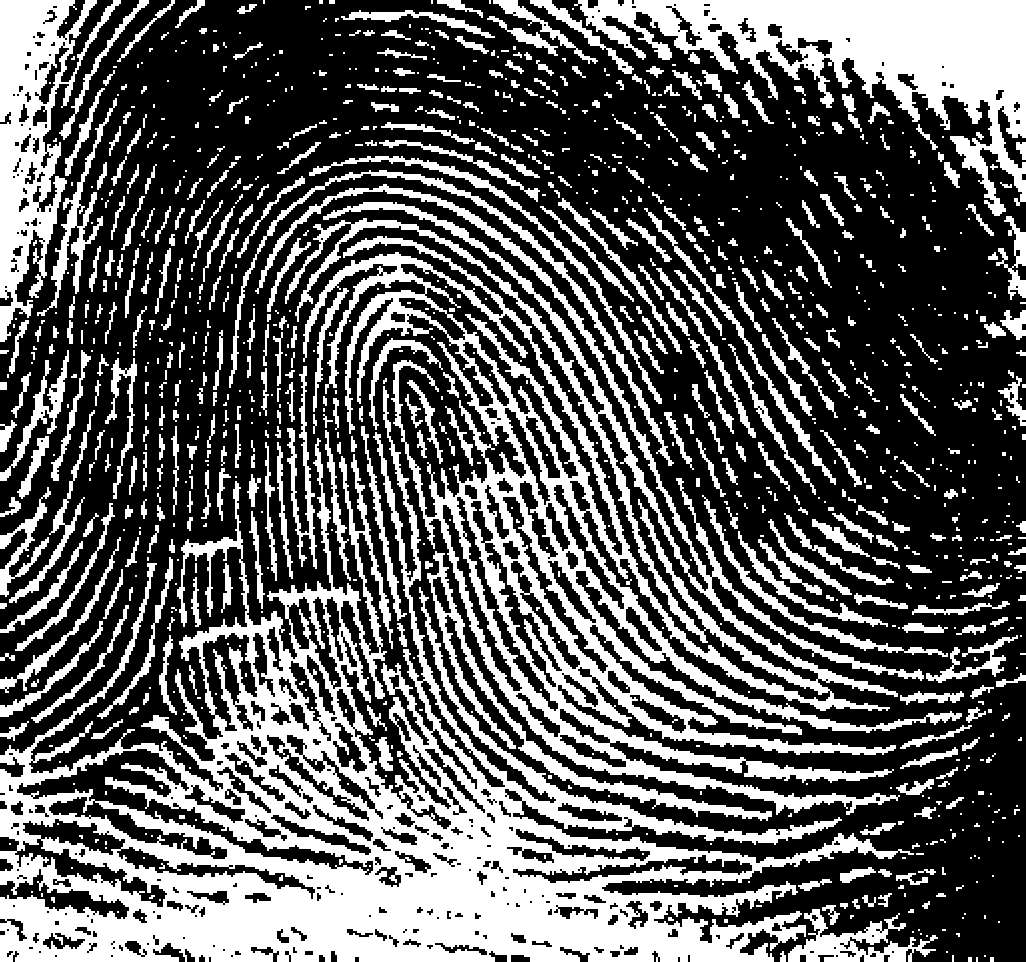
\includegraphics[width=1.00\textwidth]{figures/image_processed/thumbprint-segmented.png}
    \caption{Thumbprint segmented using Otsu's algorithm for thresholding. }
    \label{fig:thumbprint_segmented}
\end{figure}

For the result of the polymer cell, see \cref{fig:polymercell_segmented}.
\begin{figure}[]
    \centering
    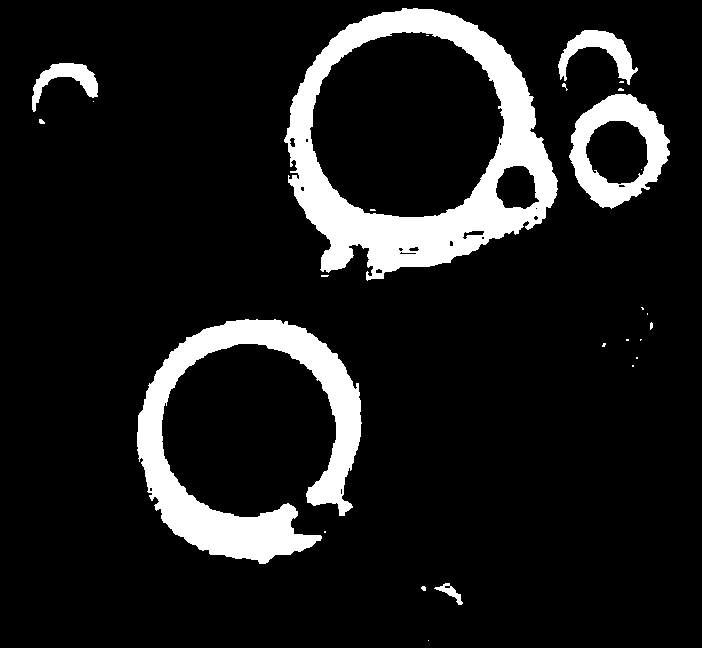
\includegraphics[width=1.00\textwidth]{figures/image_processed/polymercell-segmented.png}
    \caption{Polymer cell segmented using Otsu's algorithm for thresholding. }
    \label{fig:polymercell_segmented}
\end{figure}

\subsection{Task 3: Morphology}
\subsubsection*{a)}
Opening is particularly well suited for removing the noise / particles outside the triangle shape, as it firstly erodes information with the structuring element, then dilates the shape of the triangle back. Similarly, closing is particularly well suited for removing the noise / holes inside the triangle, as firstly the holse are dilated away, then the extra \textit{padding} added by the dilation is removed by erosion. 

See \cref{fig:noisy_filtered} for the result. The structuring element used was a disk generated from the $skimage.morphology$-library, with a radius of 7. This was the best radius I found for removing all the noise, but keeping the structure of the triangle shape. 

\begin{figure}[]
    \centering
    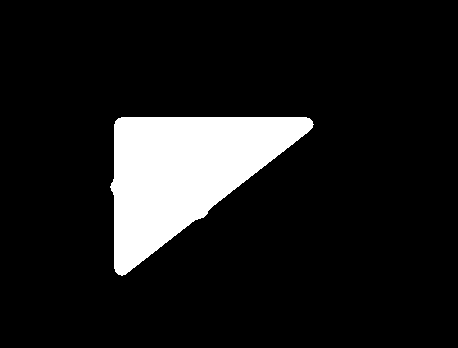
\includegraphics[width=1.00\textwidth]{figures/image_processed/noisy-filtered.png}
    \caption{Filtered version of the noisy image. }
    \label{fig:noisy_filtered}
\end{figure}


\subsubsection*{b)}
See \cref{fig:noisy_distance} for the result of the distance transform. 

\begin{figure}[]
    \centering
    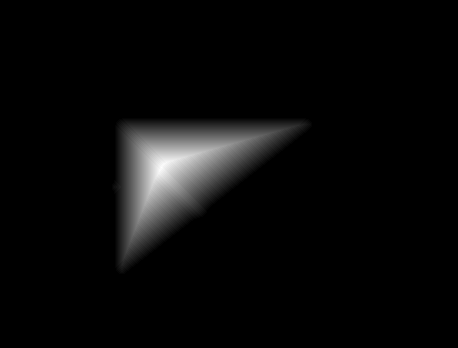
\includegraphics[width=1.00\textwidth]{figures/image_processed/noisy-distance.png}
    \caption{Distance transform of the filtered noisy triangle shape. }
    \label{fig:noisy_distance}
\end{figure}

\subsubsection*{c)}
For the resulting boundary of the image, see 

\begin{figure}[]
    \centering
    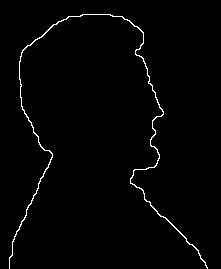
\includegraphics[width=1.00\textwidth]{figures/image_processed/lincoln-boundary.png}
    \caption{Boundary of the \textbf{lincoln.png} image. }
    \label{fig:lincoln_boundary}
\end{figure}

$(A \ominus B)$ removes the inner boundary, which we want to extract from A, then we find it by taking the difference $A - (A \ominus B)$. If we instead find the dilation $(A \oplus B)$, we will increase A by the outer boundary, and we may find this outer boundary as $(A \oplus B) - A$. 

\subsubsection*{d)}
See \cref{fig:balls_with_reflections_filled}. 

\begin{figure}[]
    \centering
    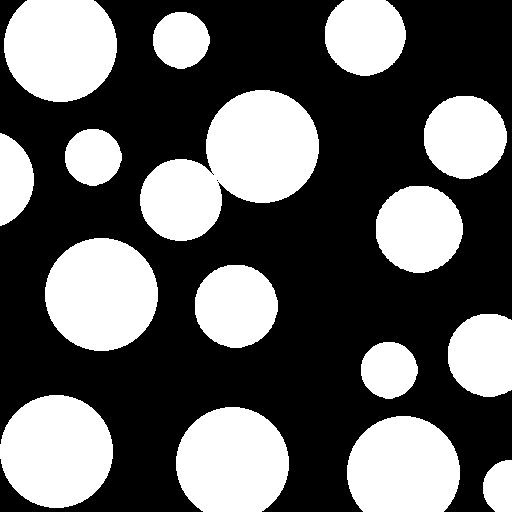
\includegraphics[width=1.00\textwidth]{figures/image_processed/balls-with-reflections-filled.png}
    \caption{Balls filled by the algorithm. }
    \label{fig:balls_with_reflections_filled}
\end{figure}
